\documentclass{ufabc}

\usepackage{amscd}
\usepackage{amsfonts}
\usepackage{amssymb}
\usepackage{epsf}
\usepackage{graphicx}
\usepackage{algorithm}
\usepackage{algpseudocode}
\usepackage{pifont}
\usepackage{indentfirst}
\usepackage{amsmath}
\usepackage[only,ninrm,elvrm,twlrm,fivrm,sixrm,sevrm,egtrm,egtit,tenrm,tenit,twlit,frtnrm]{rawfonts}

\instituicao{Universidade Federal do ABC\\Centro de Matem�tica, Computa��o e Cogni��o (CMCC)}
\curso{P�s-Gradua��o}{Ci�ncia da Computa��o}{Mestre}
\titulo{Agentes inteligentes para batalhas Pok�mon}
\autor{Jonathan Ohara}{de Araujo}
\orientador{Orientador: Prof. Dr. Fabr�cio Olivetti de Fran�a}
\coordenador{Prof. Dr. Jo�o Paulo G�is}	
\documento{Qualifica��o}
\convidados{Prof. Dr. Fabr�cio Olivetti de Fran�a}{Prof.Dr. Jo�o Paulo Gois}{Prof.Dr. Andr� Luiz Brand�o}{Prof.Dr. Denise Hideko Goya (Suplente)}
	
\date{03}{2016}

\MakeRobust{\Call}

% novos comandos para qualificacao
\newcommand{\kCC}{\emph{kCC}}
\newcommand{\kCH} {\emph{kCH}}
\newcommand{\uCC}{\emph{1CC}}
\newcommand{\uCH} {\emph{1CH}}
\newcommand{\dCC}{\emph{2CC}}
\newcommand{\dCH} {\emph{2CH}}
\newcommand{\PTH}{\mathcal{P}}
\newcommand{\Tau}{\mathcal{T}}
\newcommand{\NP}{{\rm NP}}

\begin{document}
	\maketitle

	\pagenumbering{roman}
	
%	\begin{resumo}
Esse trabalho explora a cria��o de agentes inteligentes competitivos em um ambiente onde dezenas de milhares de jogadores humanos competem diariamente para melhorar sua coloca��o no sistema de ranqueamento do jogo Pok�mon Showdown.

Escolher o melhor algoritmo e a melhor forma de aprendizado para jogar contra humanos � um dos grandes desafios desse trabalho. Outro importante aspecto que o agente precisa se adaptar � a grande variedade de composi��es de times e Pok�mons que o agente e o seu advers�rio pode montar.

Para obter a melhor flexibilidade o agente ser� submetido somente a batalhas rand�micas onde as composi��o das equipes s�o todas aleat�rias, e a avalia��o de performance do agente ser� feita atrav�s do sistema de ranqueamento do pr�prio jogo.
\end{resumo}
%	\begin{resumoingles}

To Do.

\end{resumoingles}	

	\tableofcontents
	
	\listoffigures
	
	\listoftables

	\newpage
	
	\pagenumbering{arabic}

	\chapter{�rvore de jogos}
\label{chap:arvoreDeJogos}

\section{Introdu��o}

Nesse cap�tulo vamos discutir sobre tomada de decis�o em jogos, �rvore de decis�es, �rvores de decis�es aplicadas a jogos e algoritmos baseados em �rvores.

� muito comum associar intelig�ncia para jogos, mais especificadamente intelig�ncia artificial para jogos, com a habilidade em que os elementos do jogo (jogadores n�o humanos aliados ou inimigos, objetos, fases por exemplo) tem para tomar decis�es dados certas situa��es. Apesar disso, a tomada de decis�o n�o � o �nico componente de uma intelig�ncia artificial, na se��o \ref{sec:tomadaDecisao} vamos discutir mais profundamente sobre tomada de decis�o e de outros elementos que permeiam essa �rea.

\section{Tomada de decis�o}
\label{sec:tomadaDecisao}

Tomada de decis�o � o processo de escolher uma a��o entre diversas possibilidades. Segundo \cite{introductionDecisionMaking} "Tomada de decis�o � o estudo do processo de identificar e escolher alternativas baseadas nas prefer�ncias do tomador de decis�es. Tomar uma decis�o implica que existem diferentes escolhas para serem consideradas, e, em tal caso, n�o queremos apenas identificar quais dessas alternativas s�o vi�veis, mas escolher a decis�o que melhor se encaixa com as nossas metas, objetivos, desejos, valores, e assim por diante."

Ainda na teoria do processo de tomada de decis�o, \cite{guidebookDecisionMaking} diz que o primeiro passo na tomada de decis�o � estabelecer quem �(s�o) o(s) tomador(es) de decis�o e o(s) \textit{stakeholder(s)} (partes afetadas ou interessadas), de modo a mitigar um poss�vel desacordo sobre a defini��o do problema, metas e crit�rios. O processo pode ser definidos no seguintes passos:


\begin{itemize}
	
	\item Definir o problema;
	
	\item Determinar os requisitos que a solu��o deve apresentar;

	\item Estabelecer objetivos que a solu��o do problema deve realizar;
	
	\item Identificar alternativas que ir�o solucionar o problema;
	
	\item Desenvolver crit�rios de avalia��o com base nos objetivos;
	
	\item Selecionar uma ferramenta ou m�todo para de decis�o;
	
	\item Aplicar a ferramenta ou m�todo para selecioanar a alternativa preferida;
	
	\item Validar se a resposta resolveu o problema.
	
\end{itemize}

Nos jogos, segundo \cite{Millington:2009:AIG:1795711} a entrada da tomada de decis�o � o conhecimento que tal personagem tem e a sa�da � a a��o a ser realizada. O conhecimento pode ser dividio em interno e externo. Conhecimento externo � a informa��o que o personagem tem sobre o ambiente em sua volta: posi��o dos outros personagens, o leiaute da fase, se um interruptor foi ligado, a dire��o que um barulho veio, e assim por diante. Conhecimento interno � a informa��o sobre o estado interno do personagem ou pensamentos internos como: sua sa�de, objetivos, seu passado, e assim por diante.

\section{Introdu��o MCTS}

Nesse cap�tulo vamos discutir sobre �rvore de busca de Monte Carlo (do ingl�s Monte Carlo Tree Search - MCTS) t�cnica muito utilizada para resolu��o de jogos de duas pessoas baseados em turnos. Um dos grandes problemas das �rvores de busca � o crescimento exponencial de acordo com o n�mero decis�es, pois a constru��o e a busca nessas �rvores podem levar muito tempo. O MCTS funciona muito bem para problemas onde o tempo de resposta � limitado e o espa�o de busca da �rvore pode crescer muito. Isso ocorre em batalhas Pok�mon, pegando dados de 1.000 batalhas de um dos agentes, temos que cada partida dura em m�dia 40 turnos (contando os turnos dos dois jogadores) e, em cada turno � comum ter entre 4 e 9 diferentes escolhas.

O termo Monte Carlo foi utilizado pela primeira em m�todos matem�ticos para o desenvolvimento de armas nucleares em 1940 (\cite{Kalos:1986:MCM:7050}). Segundo \cite{kleij2010monte} esse m�todo matem�tico se referia a utilizar amostras aleat�rias para estimar solu��es de problemas que eram muito dif�ceis de encontrar analiticamente. Mais tarde esse m�todo foi aplicado na computa��o e, principalmente, em �rvores de busca. O m�todo de �rvore de busca de Monte Carlo se refere a encontrar solu��es �timas em um determinado dom�nio utilizando de amostras aleat�rias no espa�o de decis�o e construindo uma �rvore de busca de acordo com os resultados (\cite{browne12asurvey}).

\section{Conceito}

A �rvore de busca de Monte Carlo � um algoritmo baseado em simula��o frequentemente usado em jogos. A ideia principal � iterativamente rodar simula��es do n� raiz da �rvore at� um n� terminal, incrementalmente crescendo uma �rvore onde o n� raiz � o estado atual do jogo (\cite{tak2014monte}).

O algoritmo de MCTS � um processo iterativo que ocorre at� que um determinado crit�rio de parada seja alcan�ado. Segundo \cite{browne12asurvey}, geralmente essa itera��o � limitada por algum recurso computacional como tempo, mem�ria ou algum contador de itera��o. No agente para Pok�mon Showdown ser� aplicado o limite de tempo, uma vez que existe um limite para cada turno.

Pode-se descrever cada itera��o do algoritmo em quatro passos b�sicos:

\begin{itemize}
	
	\item \textbf{Sele��o} Come�ando pelo n� raiz da �rvore, um n� filho � escolhido de acordo com a \textit{pol�tica de �rvore} at� que seja encontrado um \textit{n� expand�vel}. Pol�tica de �rvore � a estrat�gia de qual n� escolher, segundo \cite{browne12asurvey} essa pol�tica tem que balancear escolher n�s pouco visitados e aprofundar n�s que parecem promissores. Um n� � expand�vel quando ele n�o � n� folha e ele ainda n�o foi visitado.
	
	\item \textbf{Expans�o} � adicionado um ou mais n�s filhos no n� escolhido de acordo com as poss�veis a��es naquele estado.

	\item \textbf{Simula��o} Simula uma ou mais a��es dos novos n�s de acordo com a pol�tica padr�o para produzir uma sa�da. Pol�tica padr�o � a estrat�gia de como rodar as simula��es at� sua conclus�o.
	
	\item \textbf{Retro propaga��o} O resultado (valor) da simula��o � propagado para todos os pais do n� folha atualizando suas estat�sticas.
	
\end{itemize}

O algoritmo a seguir mostra o procedimento b�sico do MCTS:

\begin{algorithm}
\caption{Algoritmo MCTS}
\label{alg:mcts}
\begin{algorithmic}[1]
\Procedure{MCTS}{$s_{0}$}
	\State $\upsilon_{0}\gets$ criar n� raiz com estado $s_{0}$
	\While{recurso computacional}
		\State $\upsilon_{1}\gets$ \Call{Selecionar}{$\upsilon_{0}$}
		\State $s_{1}\gets$ \Call{Expandir}{$\upsilon_{1}$}
		\State $\Delta\gets$ \Call{Simular}{$s_{1}$}
		\State \Call{RetroPropagar}{$\upsilon_{1}$, $\Delta$}
	\EndWhile
	
	\State \Return $a$(\Call{MelhorFilho}{$\upsilon_{0}$})
\EndProcedure
\end{algorithmic}
\end{algorithm}

Onde:

\begin{itemize}
	
	\item $\upsilon_{0}$: N� raiz correspondente ao estado $s_{0}$.
	
	\item $\upsilon_{1}$: �ltimo n� encontrado durante a pol�tica de �rvore.
	
	\item $s_{1}$: Novo estado ap�s ocorrer a expans�o de $\upsilon_{1}$.

	\item $\Delta$: Resultado encontrado em um n�.
	
	\item $a$(\Call{MelhorFilho}{$\upsilon_{0}$}: A��o $a$ a ser tomada para alcan�ar o melhor n� filho a partir de $\upsilon_{0}$. O conceito de melhor filho varia entre as diferentes implementa��es do MCTS.
	
\end{itemize}

Na figura \ref{fig:treePolicy}(\cite{gelly2011monte}) � mostrado cinco simula��es do algoritmo MCTS e a rela��o entre a pol�tica de �rvore e pol�tica padr�o. O resultado � igual a 1 se o jogador de cor preta vencer e 0 caso branco vencer. Dentro do n� cont�m pontua��o no formato vit�ria/visitas.

\begin{figure}[p]
\centering
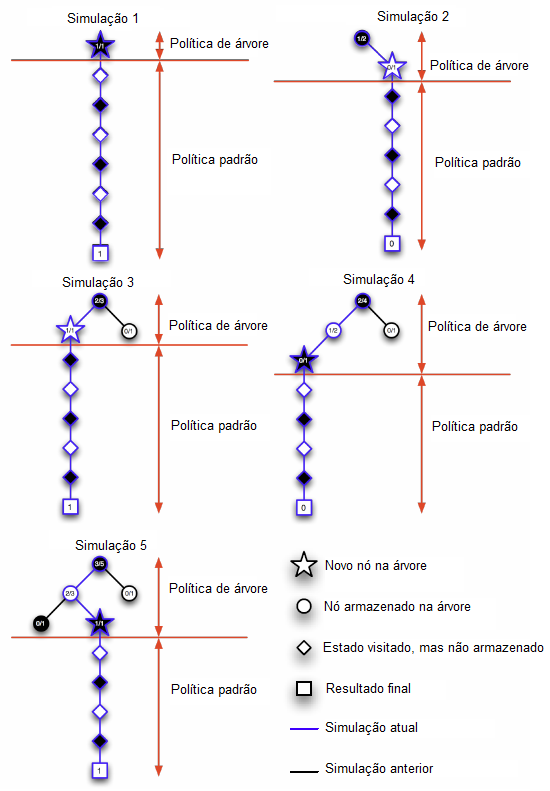
\includegraphics[width=16cm]{figures/politicasMCTS.png}
\caption[Pol�ticas MCTS]{Pol�tica de �rvore e pol�tica padr�o.}
\label{fig:treePolicy}
\end{figure}

Segundo \cite{schadd2009monte} ao finalizar o MCTS existe quatro crit�rios de como escolher o melhor filho:

\begin{itemize}
	
	\item \textbf{Filho m�ximo}: Seleciona o filho com valor mais alto.
	
	\item \textbf{Filho robusto}: Seleciona o filho com o maior n�mero de visitas.
	
	\item \textbf{Filho m�ximo-robusto}: Selecione o filho que tem tanto o maior n�mero de visita e o valor mais alto. Se n�o existir esse filho, � melhor continuar a busca at� achar um filho m�ximo-robusto do que escolher um filho com baixo n�mero de visitas.
	
	\item \textbf{Filho seguro}: Selecione o filho com menor chance de ter resultado negativo.
	
\end{itemize}

\section{Implementa��es MCTS}

A implementa��o mais popular do algoritmo MCTS � o \textit{Upper Confidence Bound for Trees} (UCT) (\cite{browne12asurvey}). Existem outras varia��es como o Online Outcome Sampling (OOS) (\cite{Lanctot2014}) ou utilizando Regret Matching junto com MCTS (\cite{tak2014monte}).	

Diferente dos jogos de turnos tradicionais onde temos turnos sequenciais uniformes, ou seja, primeiro o jogador A depois o B at� que o jogo termine, em batalhas Pok�mon as escolhas s�o feitas simultaneamente e a ordem de execu��o das a��es escolhidas depende de atributos do Pok�mon, da a��o escolhida e outros efeitos especiais. Segundo \cite{tak2014monte} o algoritmo de MCTS que obteve maior sucesso em jogos com turnos simult�neos � o UCT dissociado.

\section{Upper Confidence Bound for Trees (UCT)}

Um dos grandes dilemas na defini��o de pol�tica de �rvore � como balancear as escolhas entre explorar novos n�s para fugir de m�ximos locais e aprofundar de uma sub�rvore existente podendo achar melhores resultados ou garantindo uma maior robustez na avalia��o de um n�. Segundo \cite{auer2002finite} o Upper Confidence Bound for Trees (UCT) resolve essa quest�o de maneira �tima at� um fator constante.

O algoritmo UCT pode ser decomposto em duas partes: MCTS e Upper Confidence Bounds (UCB). Sua primeira implementa��o formal foi em 2006 por Kocsis e Szepesvari \cite{kocsis2006bandit}. O algoritmo UCB entra como uma pol�tica de �rvore para implementa��o de MCTS.


\subsection{Upper Confidence Bounds (UCB)}

O algoritmo mais tradicional de Upper Confidence Bounds � o UCB1 (\cite{auer2002finite}) que foi inicialmente aplicado para o problema \textit{multiarmed bandit}. Segundo \cite{auer2002using} o termo \textit{multiarmed bandit problem} ou problema dos ca�a-n�queis (ou mais precisamente "problema dos K ca�a-n�queis") reflete o problema de um apostador em uma sala com v�rias m�quinas de ca�a n�queis. Em cada tentativa o apostador tem que decidir em qual m�quina ele quer jogar. Para maximizar o ganho total ou recompensa, sua escolha se baseia em recompensas anteriormente coletadas em cada m�quina.

O UCB1 pode ser definido pela seguitne equacao:

\begin{equation}
UCB1 = \overline{x}_{j} + \sqrt{\frac{2 \ln n}{n_{j}}}
\end{equation}

Onde $\overline{x}_{j}$ � a m�dia da recompensa paga pela m�quina $j$, $n_{j}$ � o numero de vezes em que foi jogado na m�quina $j$ e $n$ � a soma de quantas vezes foram em jogadas em todas as m�quinas.

\subsection{Pol�tica de �rvore UCB1}

A aplica��o do UCB1 como pol�tica de �rvore funciona do seguinte modo: no processo de sele��o a escolha pode ser modelada com um problema \textit{multiarmed bandit} independente. A utilizica��o do MCTS com qualquer pol�tica de �rvore UCB � chamada de UCT.

Uma varia��o proposta por \cite{kocsis2006improved} chamada de \textit{plain UCT} provou ter resultados muito superiores ao UCT comum. Ainda segundo \cite{kocsis2006improved} com essa modifica��o a chance de selecionar o melhor movimento  converge em 1 e, atrav�s de testes emp�ricos foi observado que � mais r�pido que outros algoritmos de busca em �rvore como o \textit{alpha-beta}.

A equa��o do \textit{plain UCT} � definida da seguinte forma:

\begin{equation}
UCT = \overline{x}_{j} + 2C_{p} \sqrt{\frac{2 \ln n}{n_{j}}}
\end{equation}

Onde $C_{p} > 0$ � uma constante. O valor � sugerido como $C_{p} = \frac{1}{\sqrt{2}}$ e pode ser ajustado para mais ou menos para regular o n�vel de explora��o.

\subsection{Grupos de Movimentos}

Um aprimoramento para o UCT que foi utilizado neste trabalho � chamado de grupos de movimentos. Proposto por \cite{childs2008transpositions} essa melhoria diminui consideravelmente a quantidade de ramos da �rvore Monte Carlo. A t�cnica consiste em criar uma nova camada onde todas as poss�veis a��es s�o separadas em grupos e o UCB1 � usado para selecionar qual grupo ser� escolhido.

No agente utilizando MCTS foi aplicado nas escolhas dos jogadores. Uma vez que n�o � conhecido quais movimentos o Pok�mon advers�rio tem (cada Pok�mon pode ter apenas 4 golpes dentre dezenas de golpes que cada diferente Pok�mon pode aprender), ficaria muito custoso criar um ramo para cada poss�vel golpe de cada Pok�mon (o Pok�mon da Esp�cie Mew por exemplo, tem dispon�vel mais 120 diferentes movimentos).

Os grupos de movimentos implementados foram os seguintes:

\begin{itemize}
	
	\item \textbf{Grupo A}: Utilizar golpe de dano super efetivo. Um golpe super efetivo � um golpe que recebe um acr�scimo de $ 2 \times$ ou $ 4 \times$ de sua base de ataque de acordo com o tipo do golpe e do tipo do Pok�mon atingido (definido por um sistema de vantagens e desvantagens explicadas no cap�tulo ???).
	
	\item \textbf{Grupo B}: Utilizar outro golpe de dano qualquer.
	
	\item \textbf{Grupo C}: Utilizar golpe de altera��o de estado. Golpe de altera��o de estado podem ser golpes que enfraque�am o inimigo, fortale�a um aliado ou aplique um estado negativo (paralisar, envenenar e etc).
	
	\item \textbf{Grupo D}: Trocar para algum Pok�mon que tenha algum golpe super efetivo (Grupo A) contra o atual inimigo.
	
	\item \textbf{Grupo E}: Trocar para outro Pok�mon qualquer.
	
\end{itemize}

Antes de cada poss�vel golpe ser encaixado em cada grupo � verificado a imunidade do Pok�mon advers�rio a esse golpe. Caso o Pok�mon advers�rio seja imune ou o golpe n�o tenha efeito (como por exemplo, curar quando os pontos de vidas j� est�o 100\%, tentar aplicar o estado de paraliza��o em um Pok�mon j� paralisado, entre outros) o movimento � descartado n�o entrando para nenhum grupo.

Caso um grupo n�o contenha nenhuma a��o o grupo � descartado da fase de sele��o e expans�o do MCTS. No caso de existir mais de uma a��o, a escolha � feita diferente para cada grupo, conforme as seguintes regras:

\begin{itemize}
	
	\item \textbf{Grupo A e B}: � definido por qual golpe tem maior dano bruto (dano antes das redu��es). Definido pela equa��o:
	
	\begin{equation}
		danobruto = efetividade \times stab \times baseforca
	\end{equation}
	
	Onde:
	
		\subitem \textbf{efetividade}: $\frac{1}{4}$ (super n�o efetivo), $\frac{1}{2}$ (n�o efetivo), $1$, $2$ (efetivo) e $4$ (super efetivo).
		
		\subitem \textbf{stab}: $1$ caso o tipo do Pok�mon seja diferente do tipo do golpe e $2$ caso sejam do mesmo tipo.
		
		\subitem \textbf{baseforca}: For�a base do golpe.
	
	\item \textbf{Grupo C}: Escolhido aleatoriamente.
	
	\item \textbf{Grupo D e E}: Maior quantidade de HP e depois a maior quantidade do atributo velocidade.
	
\end{itemize}

	\bibliographystyle{apalike}	
	\bibliography{Bibliografia}

\end{document}